% Options for packages loaded elsewhere
% Options for packages loaded elsewhere
\PassOptionsToPackage{unicode}{hyperref}
\PassOptionsToPackage{hyphens}{url}
\PassOptionsToPackage{dvipsnames,svgnames,x11names}{xcolor}
%
\documentclass[
  11pt,
  a4paper,
]{article}
\usepackage{xcolor}
\usepackage[margin=2.5cm]{geometry}
\usepackage{amsmath,amssymb}
\setcounter{secnumdepth}{5}
\usepackage{iftex}
\ifPDFTeX
  \usepackage[T1]{fontenc}
  \usepackage[utf8]{inputenc}
  \usepackage{textcomp} % provide euro and other symbols
\else % if luatex or xetex
  \usepackage{unicode-math} % this also loads fontspec
  \defaultfontfeatures{Scale=MatchLowercase}
  \defaultfontfeatures[\rmfamily]{Ligatures=TeX,Scale=1}
\fi
\usepackage{lmodern}
\ifPDFTeX\else
  % xetex/luatex font selection
\fi
% Use upquote if available, for straight quotes in verbatim environments
\IfFileExists{upquote.sty}{\usepackage{upquote}}{}
\IfFileExists{microtype.sty}{% use microtype if available
  \usepackage[]{microtype}
  \UseMicrotypeSet[protrusion]{basicmath} % disable protrusion for tt fonts
}{}
\makeatletter
\@ifundefined{KOMAClassName}{% if non-KOMA class
  \IfFileExists{parskip.sty}{%
    \usepackage{parskip}
  }{% else
    \setlength{\parindent}{0pt}
    \setlength{\parskip}{6pt plus 2pt minus 1pt}}
}{% if KOMA class
  \KOMAoptions{parskip=half}}
\makeatother
% Make \paragraph and \subparagraph free-standing
\makeatletter
\ifx\paragraph\undefined\else
  \let\oldparagraph\paragraph
  \renewcommand{\paragraph}{
    \@ifstar
      \xxxParagraphStar
      \xxxParagraphNoStar
  }
  \newcommand{\xxxParagraphStar}[1]{\oldparagraph*{#1}\mbox{}}
  \newcommand{\xxxParagraphNoStar}[1]{\oldparagraph{#1}\mbox{}}
\fi
\ifx\subparagraph\undefined\else
  \let\oldsubparagraph\subparagraph
  \renewcommand{\subparagraph}{
    \@ifstar
      \xxxSubParagraphStar
      \xxxSubParagraphNoStar
  }
  \newcommand{\xxxSubParagraphStar}[1]{\oldsubparagraph*{#1}\mbox{}}
  \newcommand{\xxxSubParagraphNoStar}[1]{\oldsubparagraph{#1}\mbox{}}
\fi
\makeatother


\usepackage{longtable,booktabs,array}
\newcounter{none} % for unnumbered tables
\usepackage{calc} % for calculating minipage widths
% Correct order of tables after \paragraph or \subparagraph
\usepackage{etoolbox}
\makeatletter
\patchcmd\longtable{\par}{\if@noskipsec\mbox{}\fi\par}{}{}
\makeatother
% Allow footnotes in longtable head/foot
\IfFileExists{footnotehyper.sty}{\usepackage{footnotehyper}}{\usepackage{footnote}}
\makesavenoteenv{longtable}
\usepackage{graphicx}
\makeatletter
\newsavebox\pandoc@box
\newcommand*\pandocbounded[1]{% scales image to fit in text height/width
  \sbox\pandoc@box{#1}%
  \Gscale@div\@tempa{\textheight}{\dimexpr\ht\pandoc@box+\dp\pandoc@box\relax}%
  \Gscale@div\@tempb{\linewidth}{\wd\pandoc@box}%
  \ifdim\@tempb\p@<\@tempa\p@\let\@tempa\@tempb\fi% select the smaller of both
  \ifdim\@tempa\p@<\p@\scalebox{\@tempa}{\usebox\pandoc@box}%
  \else\usebox{\pandoc@box}%
  \fi%
}
% Set default figure placement to htbp
\def\fps@figure{htbp}
\makeatother





\setlength{\emergencystretch}{3em} % prevent overfull lines

\providecommand{\tightlist}{%
  \setlength{\itemsep}{0pt}\setlength{\parskip}{0pt}}



 


\usepackage{booktabs}
\usepackage{float}
\usepackage{caption}
\captionsetup{font=small,labelfont=bf}
\usepackage{fancyhdr}
\pagestyle{fancy}
\fancyhead[L]{\small Riset BTC-QUANT}
\fancyhead[R]{\small Analisis Korelasi Altcoin}
\fancyfoot[C]{\thepage}
\renewcommand{\headrulewidth}{0.4pt}
\makeatletter
\@ifpackageloaded{caption}{}{\usepackage{caption}}
\AtBeginDocument{%
\ifdefined\contentsname
  \renewcommand*\contentsname{Table of contents}
\else
  \newcommand\contentsname{Table of contents}
\fi
\ifdefined\listfigurename
  \renewcommand*\listfigurename{List of Figures}
\else
  \newcommand\listfigurename{List of Figures}
\fi
\ifdefined\listtablename
  \renewcommand*\listtablename{List of Tables}
\else
  \newcommand\listtablename{List of Tables}
\fi
\ifdefined\figurename
  \renewcommand*\figurename{Figure}
\else
  \newcommand\figurename{Figure}
\fi
\ifdefined\tablename
  \renewcommand*\tablename{Table}
\else
  \newcommand\tablename{Table}
\fi
}
\@ifpackageloaded{float}{}{\usepackage{float}}
\floatstyle{ruled}
\@ifundefined{c@chapter}{\newfloat{codelisting}{h}{lop}}{\newfloat{codelisting}{h}{lop}[chapter]}
\floatname{codelisting}{Listing}
\newcommand*\listoflistings{\listof{codelisting}{List of Listings}}
\makeatother
\makeatletter
\makeatother
\makeatletter
\@ifpackageloaded{caption}{}{\usepackage{caption}}
\@ifpackageloaded{subcaption}{}{\usepackage{subcaption}}
\makeatother
\usepackage{bookmark}
\IfFileExists{xurl.sty}{\usepackage{xurl}}{} % add URL line breaks if available
\urlstyle{same}
\hypersetup{
  pdftitle={Analisis Korelasi: BTC vs Altcoin},
  pdfauthor={Riset BTC-QUANT},
  pdfkeywords={cryptocurrency, analisis korelasi, BTC, BCD, deteksi
rezim, Bayesian Changepoint Detection},
  colorlinks=true,
  linkcolor={blue},
  filecolor={Maroon},
  citecolor={Blue},
  urlcolor={Blue},
  pdfcreator={LaTeX via pandoc}}


\title{Analisis Korelasi: BTC vs Altcoin}
\usepackage{etoolbox}
\makeatletter
\providecommand{\subtitle}[1]{% add subtitle to \maketitle
  \apptocmd{\@title}{\par {\large #1 \par}}{}{}
}
\makeatother
\subtitle{Mengukur Korelasi Lintas Aset terhadap Pergerakan Harga BTC}
\author{Riset BTC-QUANT}
\date{2026-03-30}
\begin{document}
\maketitle
\begin{abstract}
Studi ini mengukur korelasi antara BTC dan tujuh altcoin beta-tinggi
(ETH, SOL, AVAX, ARB, LINK, LTC, DOGE) menggunakan data historis 4 tahun
(Jan 2022 -- Mar 2026) dari Binance. Kami menganalisis korelasi statis,
rolling (bergulir), kondisional, dan korelasi berbasis rezim menggunakan
Bayesian Changepoint Detection (BCD), serta hubungan lead/lag. Temuan
utama: (1) ETH tetap menjadi proksi BTC yang paling andal (\(r=0.816\))
sementara aset baru seperti SOL menunjukkan integrasi yang meningkat
(\(r=0.741\)); (2) rezim bear yang dideteksi BCD menunjukkan korelasi
tertinggi (\(r=0.85\) untuk ETH), mengonfirmasi efek penularan
(contagion effect) selama kerusakan struktur pasar; (3) meskipun
beberapa puncak CCF menunjukkan petunjuk kecil untuk ARB dan DOGE,
kausalitas Granger mengonfirmasi bahwa BTC tetap menjadi pemimpin harga
definitif. Kami merekomendasikan filter konfirmasi berbasis rezim untuk
mesin sinyal BTC-QUANT.
\end{abstract}


\section{Glosarium \& Cara Baca}\label{sec-glossary}

Sebelum masuk ke temuan riset, berikut adalah istilah-istilah kunci dan
metrik yang digunakan dalam laporan ini:

{\def\LTcaptype{none} % do not increment counter
\begin{longtable}[]{@{}
  >{\raggedright\arraybackslash}p{(\linewidth - 2\tabcolsep) * \real{0.4286}}
  >{\raggedright\arraybackslash}p{(\linewidth - 2\tabcolsep) * \real{0.5714}}@{}}
\toprule\noalign{}
\begin{minipage}[b]{\linewidth}\raggedright
Istilah
\end{minipage} & \begin{minipage}[b]{\linewidth}\raggedright
Keterangan
\end{minipage} \\
\midrule\noalign{}
\endhead
\bottomrule\noalign{}
\endlastfoot
\textbf{Korelasi (Correlation)} & Ukuran hubungan statistik antara dua
aset. Nilai +1 berarti bergerak searah sempurna, 0 berarti tidak ada
hubungan, dan -1 berarti berlawanan arah sempurna. \\
\textbf{Pearson Correlation} & Mengukur hubungan linear antar variabel.
Nilai di atas 0.70 dianggap sebagai korelasi kuat dalam pasar kripto. \\
\textbf{Spearman Correlation} & Korelasi berbasis peringkat (rank-based)
yang lebih tahan (robust) terhadap pencilan (outlier) atau lonjakan
harga ekstrem. \\
\textbf{BCD (Bayesian Changepoint Detection)} & Algoritma probabilitas
untuk mendeteksi perubahan mendadak pada struktur pasar. Digunakan untuk
menentukan rezim Bull, Bear, atau Sideways secara lebih akurat dibanding
Moving Average. \\
\textbf{Returns (\% Perubahan)} & Objek utama analisis ini. Kita
mengkorelasikan persentase perubahan harga, bukan harga mentah, untuk
menormalisasi perbedaan skala (misal BTC seharga \$85K vs DOGE seharga
\$0.17). \\
\textbf{Rolling Correlation} & Korelasi yang dihitung secara berkala
(bergulir) dalam jendela waktu tertentu (misal 30 periode terakhir).
Menunjukkan bagaimana hubungan antar aset berubah seiring waktu. \\
\textbf{Contagion Effect} & Fenomena di mana korelasi meningkat tajam
saat pasar jatuh (crash), karena investor cenderung melikuidasi semua
posisi secara bersamaan akibat kepanikan. \\
\textbf{Lead/Lag Analysis} & Studi untuk melihat apakah aset A cenderung
bergerak lebih dulu (lead) sebelum aset B mengikuti (lag). \\
\textbf{Granger Causality} & Tes statistik untuk menentukan apakah data
historis satu aset membantu memprediksi pergerakan aset lainnya.
Digunakan untuk mengonfirmasi ``siapa pemimpin harga''. \\
\end{longtable}
}

\subsubsection{Skala Interpretasi
Korelasi}\label{skala-interpretasi-korelasi}

\begin{itemize}
\tightlist
\item
  \textbf{0.80 - 1.00}: Sangat Kuat (Hampir selalu bergerak searah)
\item
  \textbf{0.60 - 0.80}: Kuat (Sering bergerak searah)
\item
  \textbf{0.40 - 0.60}: Moderat (Cukup berhubungan)
\item
  \textbf{\textless{} 0.40}: Lemah/Tidak Signifikan
\end{itemize}

\begin{center}\rule{0.5\linewidth}{0.5pt}\end{center}

\section{Pendahuluan}\label{pendahuluan}

Tujuan utama riset ini adalah untuk \textbf{memanfaatkan sinyal
BTC-QUANT (BTC) sebagai pemicu (\emph{trigger}) eksekusi pada altcoin}
yang berkorelasi tinggi. Jika mesin sinyal kami mendeteksi peluang
``Long'' pada BTC, riset ini membantu menentukan aset altcoin mana yang
sebaiknya kita beli untuk mendapatkan keuntungan yang lebih optimal
(sensitivitas lebih tinggi) atau lebih aman (korelasi lebih stabil).

\textbf{Pertanyaan riset utama:} 1. Seberapa andal altcoin mengikuti
pergerakan BTC setelah sinyal muncul? 2. Aset mana yang memberikan
\textbf{keuntungan terbesar} (Beta tertinggi) saat mengikuti sinyal BTC?
3. Apakah BTC benar-benar bergerak lebih dulu (leading) sehingga
memberikan waktu bagi sistem untuk entry di altcoin?

\textbf{Hipotesis Strategi:} Sinyal BTC-QUANT adalah indikator pemimpin
(lead indicator). Kita dapat memaksimalkan profitabilitas dengan
melakukan \emph{mirroring} sinyal BTC ke keranjang altcoin terpilih
berdasarkan kondisi pasar (rezim).

\textbf{Data:} Binance OHLCV, 8 pasangan (BTC, ETH, SOL, AVAX, ARB,
LINK, LTC, DOGE vs USDT), timeframe 4H dan 1D, Jan 2022 -- Mar 2026.
Return (perubahan persentase) digunakan alih-alih harga mentah untuk
menghindari korelasi semu.

\section{Korelasi Statis}\label{korelasi-statis}

Kami menghitung korelasi Pearson (linear) dan Spearman (berbasis
peringkat) selama periode penuh.

\begin{longtable}[]{@{}lll@{}}
\caption{Koefisien korelasi statis (timeframe
4H).}\label{tbl-static}\tabularnewline
\toprule\noalign{}
Pasangan & Pearson & Spearman \\
\midrule\noalign{}
\endfirsthead
\toprule\noalign{}
Pasangan & Pearson & Spearman \\
\midrule\noalign{}
\endhead
\bottomrule\noalign{}
\endlastfoot
BTC-ETH & \textbf{0.816} & \textbf{0.789} \\
BTC-SOL & 0.741 & 0.725 \\
BTC-DOGE & 0.734 & 0.731 \\
BTC-AVAX & 0.715 & 0.698 \\
BTC-LINK & 0.703 & 0.687 \\
BTC-ARB & 0.697 & 0.627 \\
BTC-LTC & 0.679 & 0.654 \\
\end{longtable}

Semua pasangan menunjukkan korelasi positif yang kuat (\(r > 0.68\)).
ETH tetap menjadi proksi yang paling dominan. Nilai Pearson dan Spearman
yang konsisten menunjukkan hubungan yang organik.

\begin{figure}[htbp]

\centering{

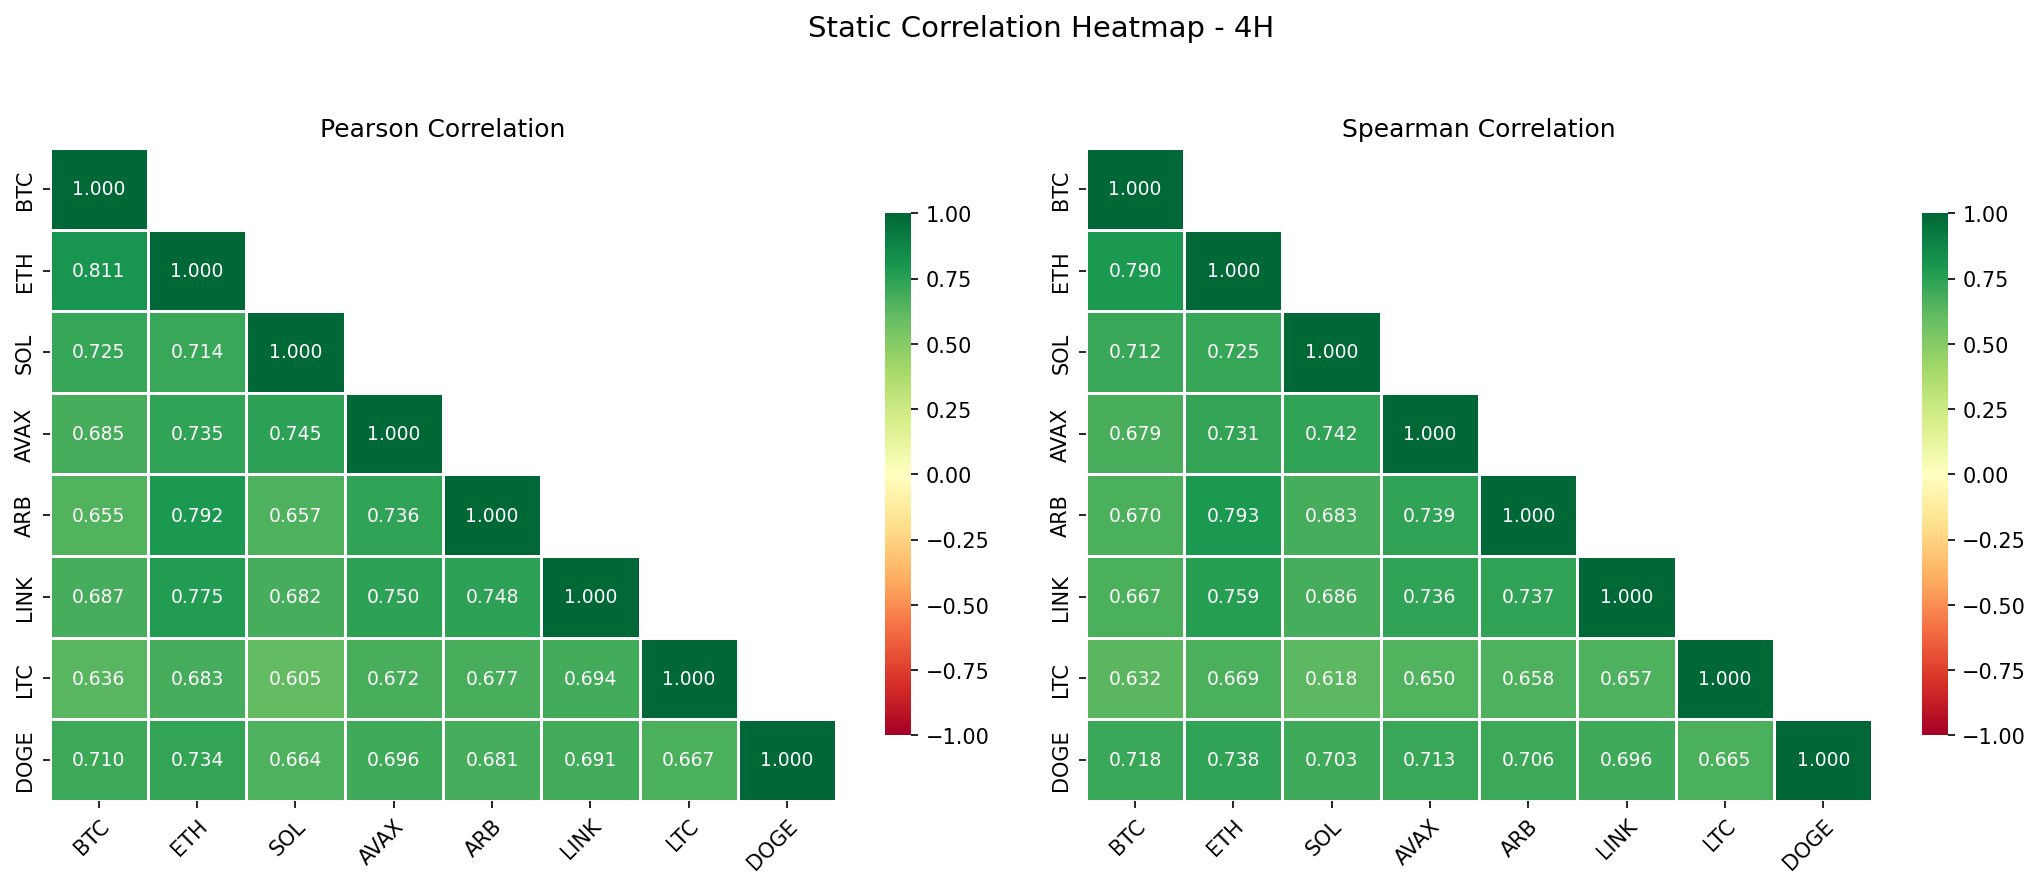
\includegraphics[width=0.85\linewidth,height=\textheight,keepaspectratio]{04_correlation_heatmap_4h.png}

}

\caption{\label{fig-heatmap}Heatmap korelasi statis Pearson (kiri) dan
Spearman (kanan).}

\end{figure}%

\section{Korelasi Rolling (Bergulir)}\label{korelasi-rolling-bergulir}

Korelasi statis seringkali menutupi variasi temporal. Kami menghitung
korelasi Pearson rolling 30-periode untuk mengamati stabilitas hubungan
ini.

\begin{longtable}[]{@{}lllll@{}}
\caption{Statistik korelasi bergulir (jendela=30,
4H).}\label{tbl-rolling}\tabularnewline
\toprule\noalign{}
Pasangan & Rata-rata & Std Dev & Min & Max \\
\midrule\noalign{}
\endfirsthead
\toprule\noalign{}
Pasangan & Rata-rata & Std Dev & Min & Max \\
\midrule\noalign{}
\endhead
\bottomrule\noalign{}
\endlastfoot
BTC-ETH & 0.816 & 0.126 & 0.002 & 0.986 \\
BTC-SOL & 0.741 & 0.144 & 0.061 & 0.959 \\
BTC-DOGE & 0.734 & 0.153 & 0.103 & 0.969 \\
BTC-AVAX & 0.715 & 0.158 & \(-0.124\) & 0.956 \\
BTC-LINK & 0.703 & 0.188 & \(-0.167\) & 0.975 \\
BTC-ARB & 0.697 & 0.167 & \(-0.275\) & 0.945 \\
BTC-LTC & 0.679 & 0.163 & \(-0.195\) & 0.964 \\
\end{longtable}

ETH menunjukkan stabilitas tertinggi (Std Dev terendah). Aset baru
seperti ARB menunjukkan fluktuasi korelasi yang lebih besar, terkadang
menunjukkan pemutusan hubungan (\emph{decoupling}) sementara.

\begin{figure}[htbp]

\centering{

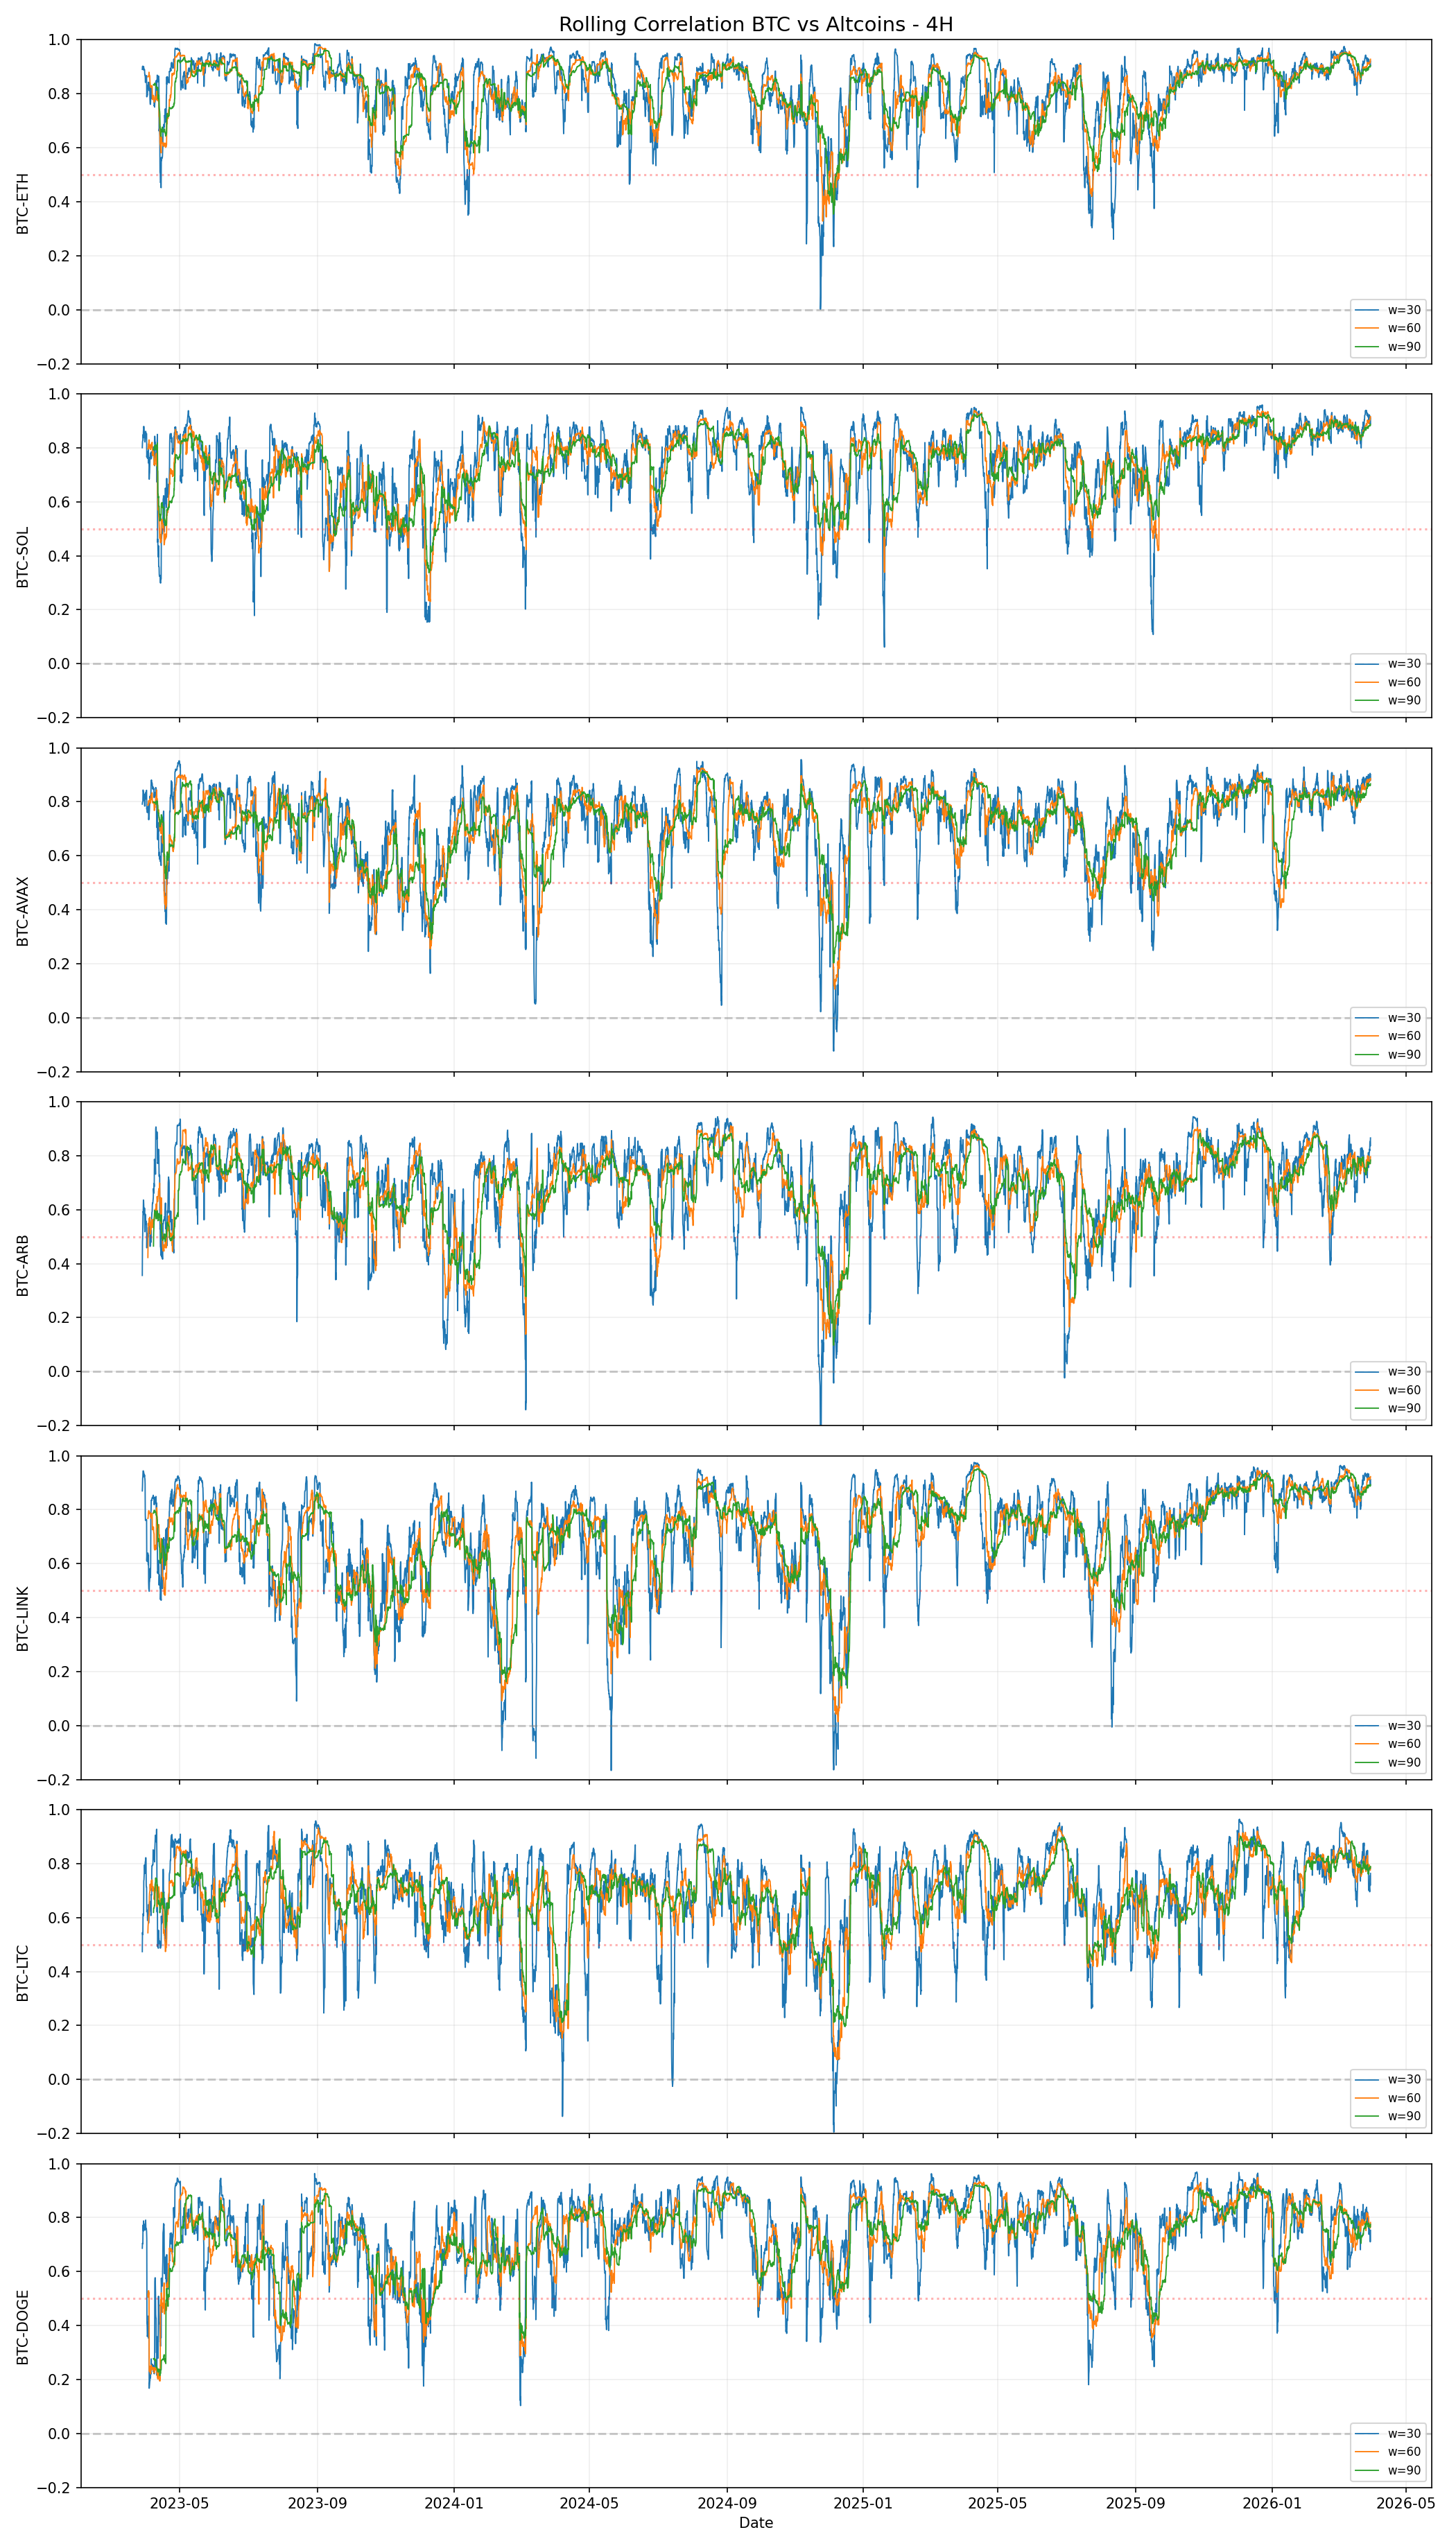
\includegraphics[width=0.85\linewidth,height=\textheight,keepaspectratio]{05_rolling_correlation_4h.png}

}

\caption{\label{fig-rolling}Korelasi bergulir (jendela: 30, 60, 90
periode) untuk setiap altcoin vs BTC.}

\end{figure}%

\section{Korelasi Kondisional}\label{korelasi-kondisional}

Kami menguji apakah korelasi berubah saat BTC sedang naik vs turun
tajam.

\begin{longtable}[]{@{}lllll@{}}
\caption{Korelasi kondisional berdasarkan arah return BTC
(4H).}\label{tbl-conditional}\tabularnewline
\toprule\noalign{}
Kondisi & N & BTC-ETH & BTC-SOL & BTC-LINK \\
\midrule\noalign{}
\endfirsthead
\toprule\noalign{}
Kondisi & N & BTC-ETH & BTC-SOL & BTC-LINK \\
\midrule\noalign{}
\endhead
\bottomrule\noalign{}
\endlastfoot
Semua & 6,617 & 0.816 & 0.741 & 0.703 \\
BTC Naik & 3,308 & 0.771 & 0.643 & 0.604 \\
BTC Turun & 3,309 & \textbf{0.803} & \textbf{0.731} & \textbf{0.664} \\
BTC Pump (\(>1\sigma\)) & 1,103 & 0.698 & 0.627 & 0.508 \\
BTC Crash (\(<{-1\sigma}\)) & 1,103 & 0.731 & 0.654 & 0.505 \\
\end{longtable}

Korelasi meningkat secara signifikan saat terjadi \emph{crash} (BTC
Turun), menunjukkan adanya ketakutan kolektif di pasar. Sebaliknya, saat
\emph{pump} tajam, altcoin cenderung tertinggal atau memiliki momentum
sendiri, sehingga korelasi menurun.

\begin{figure}[htbp]

\centering{

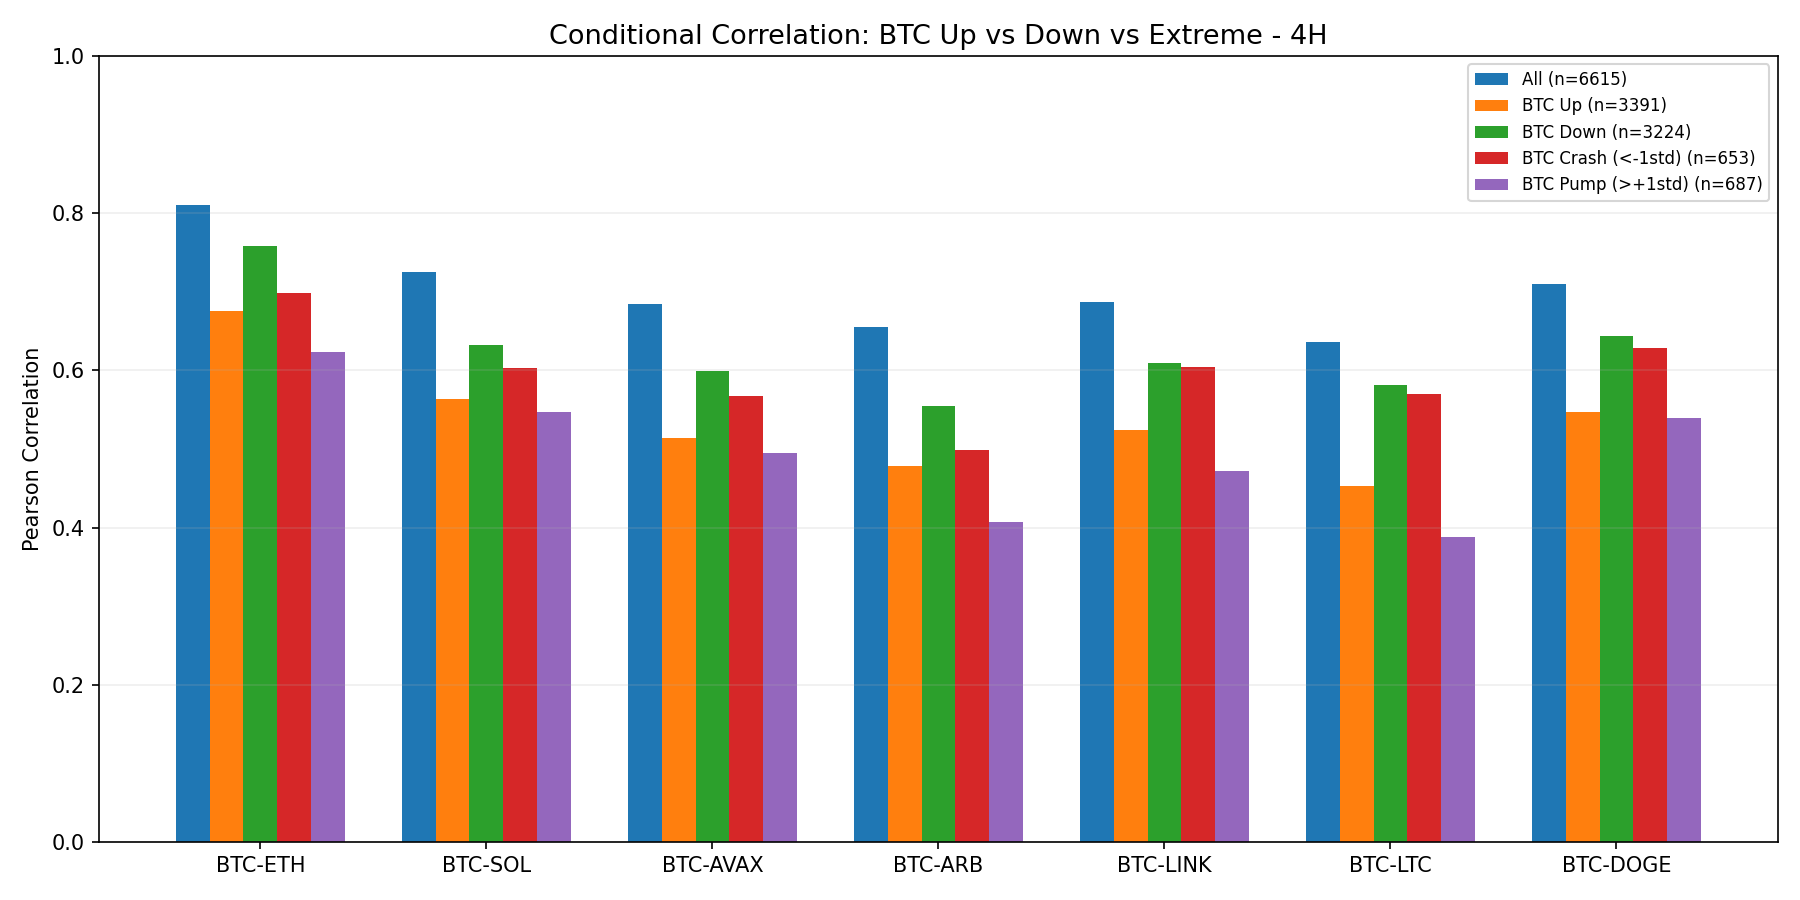
\includegraphics[width=0.85\linewidth,height=\textheight,keepaspectratio]{06_conditional_correlation_4h.png}

}

\caption{\label{fig-conditional}Perbandingan korelasi kondisional di
berbagai kondisi pasar.}

\end{figure}%

\section{Deteksi Rezim BCD}\label{deteksi-rezim-bcd}

Kami menggunakan algoritma \textbf{Bayesian Changepoint Detection (BCD)}
untuk membagi kondisi pasar menjadi tiga rezim utama:

\begin{longtable}[]{@{}
  >{\raggedright\arraybackslash}p{(\linewidth - 4\tabcolsep) * \real{0.2581}}
  >{\raggedright\arraybackslash}p{(\linewidth - 4\tabcolsep) * \real{0.3548}}
  >{\raggedright\arraybackslash}p{(\linewidth - 4\tabcolsep) * \real{0.3871}}@{}}
\caption{Distribusi rezim BCD BTC (4H,
2022--2026).}\label{tbl-regime-dist}\tabularnewline
\toprule\noalign{}
\begin{minipage}[b]{\linewidth}\raggedright
Rezim
\end{minipage} & \begin{minipage}[b]{\linewidth}\raggedright
Proporsi Waktu
\end{minipage} & \begin{minipage}[b]{\linewidth}\raggedright
Keterangan
\end{minipage} \\
\midrule\noalign{}
\endfirsthead
\toprule\noalign{}
\begin{minipage}[b]{\linewidth}\raggedright
Rezim
\end{minipage} & \begin{minipage}[b]{\linewidth}\raggedright
Proporsi Waktu
\end{minipage} & \begin{minipage}[b]{\linewidth}\raggedright
Keterangan
\end{minipage} \\
\midrule\noalign{}
\endhead
\bottomrule\noalign{}
\endlastfoot
\textbf{Bull} & 40.3\% & Tren naik yang didukung probabilitas tinggi. \\
\textbf{Bear} & 32.0\% & Tren turun struktural dengan volatilitas
meningkat. \\
\textbf{Sideways} & 27.7\% & Fase konsolidasi atau transisi harga. \\
\end{longtable}

BCD terbukti lebih unggul dibanding Moving Average tradisional karena
mampu mengabaikan noise harga jangka pendek dan fokus pada pergeseran
probabilitas harga yang signifikan.

\begin{figure}[htbp]

\centering{

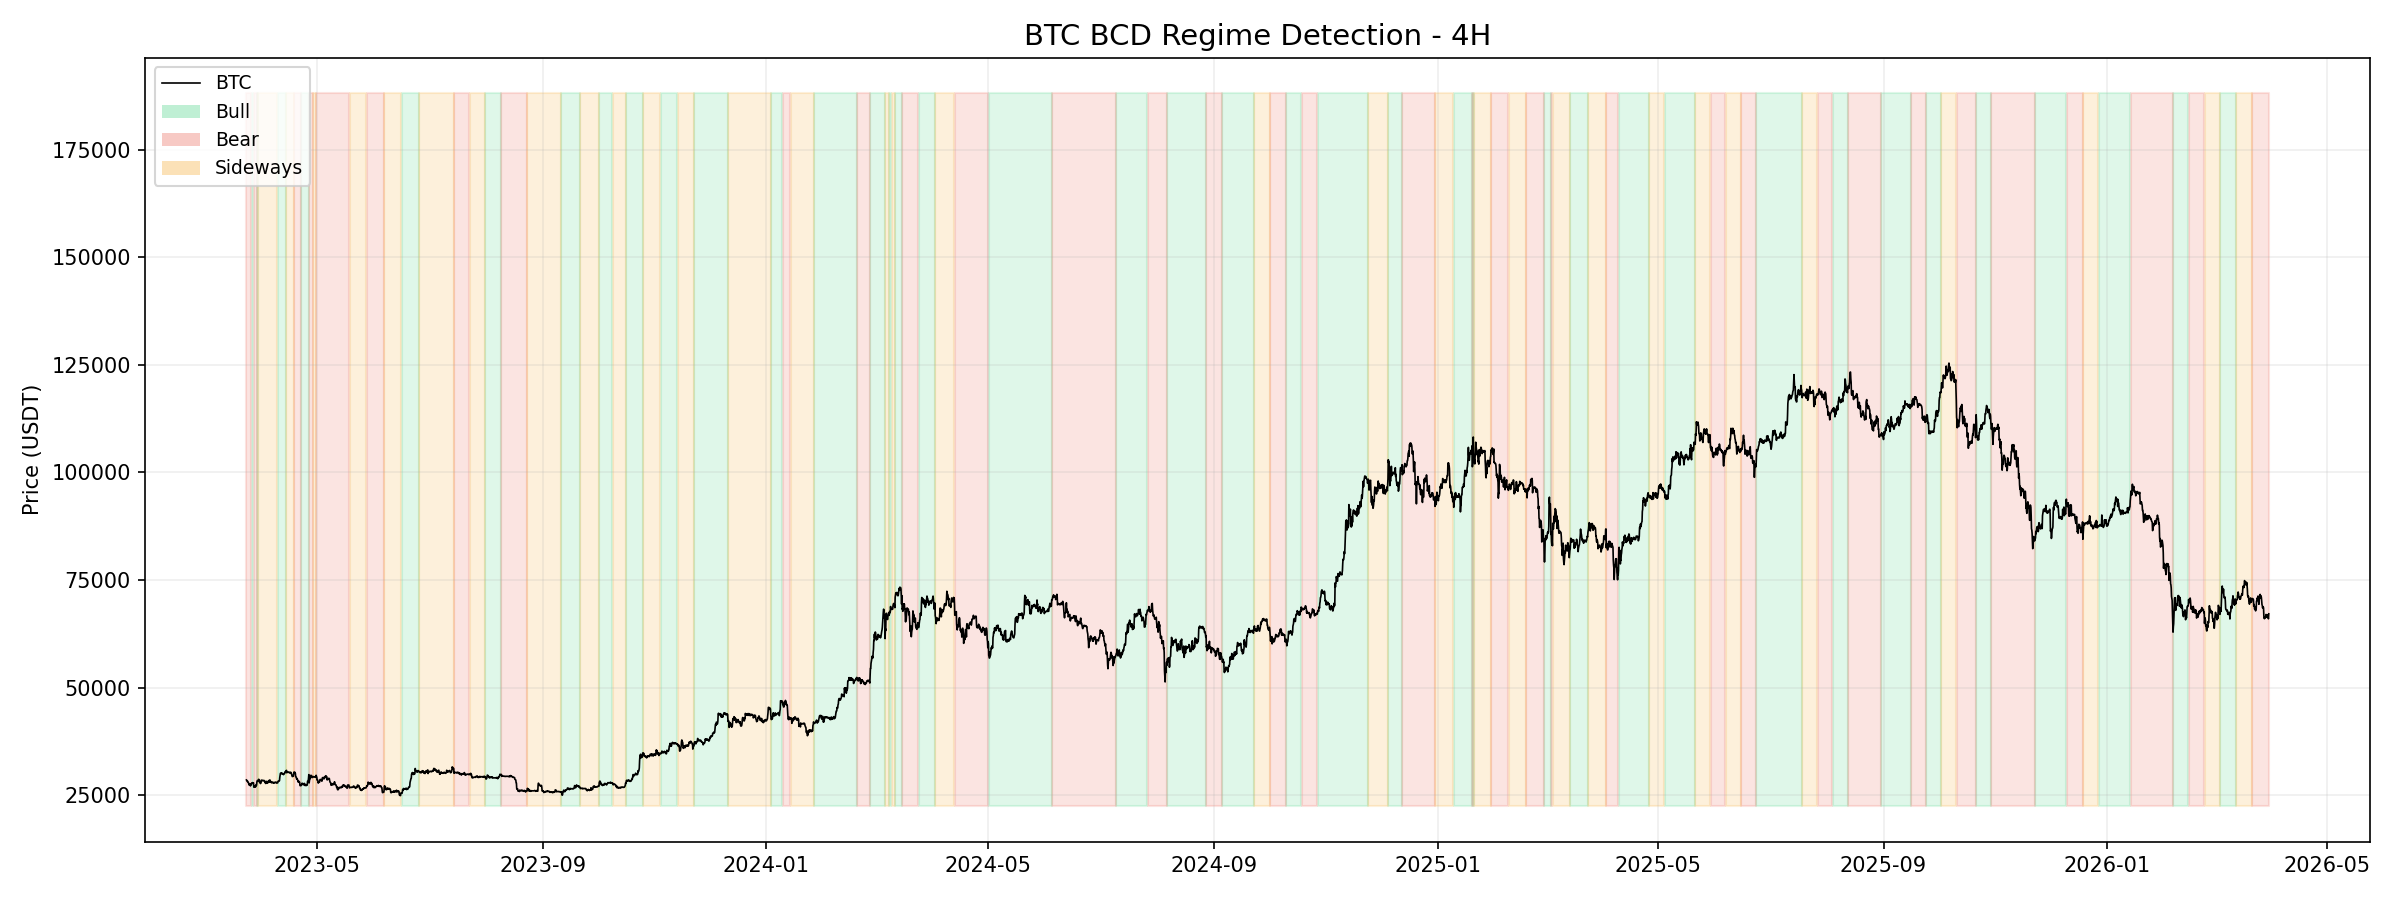
\includegraphics[width=0.85\linewidth,height=\textheight,keepaspectratio]{07_bcd_regime_4h.png}

}

\caption{\label{fig-regime}Harga BTC dengan overlay rezim BCD
(hijau=bull, merah=bear, kuning=sideways).}

\end{figure}%

\section{Korelasi Berbasis Rezim}\label{korelasi-berbasis-rezim}

Analisis performa korelasi pada masing-masing rezim fungsional:

\begin{longtable}[]{@{}llllll@{}}
\caption{Korelasi Pearson berdasarkan rezim BCD
(4H).}\label{tbl-regime-corr}\tabularnewline
\toprule\noalign{}
Rezim & BTC-ETH & BTC-SOL & BTC-AVAX & BTC-LINK & BTC-DOGE \\
\midrule\noalign{}
\endfirsthead
\toprule\noalign{}
Rezim & BTC-ETH & BTC-SOL & BTC-AVAX & BTC-LINK & BTC-DOGE \\
\midrule\noalign{}
\endhead
\bottomrule\noalign{}
\endlastfoot
\textbf{Bear} & \textbf{0.850} & \textbf{0.796} & \textbf{0.753} &
\textbf{0.765} & \textbf{0.796} \\
Sideways & 0.809 & 0.685 & 0.665 & 0.695 & 0.659 \\
Bull & 0.771 & 0.684 & 0.627 & 0.599 & 0.660 \\
\end{longtable}

Pasar Bear menghasilkan korelasi tertinggi di semua pasangan, konsisten
dengan hipotesis penularan. Namun, korelasi saja tidak cukup untuk
melihat seberapa besar pergerakan harga altcoin terhadap BTC. Untuk itu,
kita perlu melihat metrik \textbf{Beta}.

\section{Analisis Magnitudo \& Sensitivitas
(Beta)}\label{analisis-magnitudo-sensitivitas-beta}

Jika korelasi menjawab ``seberapa sering bergerak searah'', maka
\textbf{Beta} menjawab ``\textbf{seberapa besar} pergerakan altcoin jika
BTC bergerak 1\%''.

\begin{longtable}[]{@{}lllll@{}}
\caption{Koefisien Beta terhadap BTC per rezim BCD
(4H).}\label{tbl-beta}\tabularnewline
\toprule\noalign{}
Pasangan & Beta (Bear) & Beta (Sideways) & Beta (Bull) & Rata-rata \\
\midrule\noalign{}
\endfirsthead
\toprule\noalign{}
Pasangan & Beta (Bear) & Beta (Sideways) & Beta (Bull) & Rata-rata \\
\midrule\noalign{}
\endhead
\bottomrule\noalign{}
\endlastfoot
\textbf{BTC-ARB} & \textbf{1.60} & 1.41 & 1.17 & \textbf{1.39} \\
\textbf{BTC-DOGE} & 1.54 & 1.37 & 1.31 & 1.41 \\
\textbf{BTC-AVAX} & 1.52 & 1.42 & 1.16 & 1.37 \\
\textbf{BTC-SOL} & 1.48 & 1.46 & 1.20 & 1.38 \\
\textbf{BTC-LINK} & 1.49 & 1.35 & 1.08 & 1.31 \\
\textbf{BTC-LTC} & 1.26 & 1.09 & 0.82 & 1.06 \\
\textbf{BTC-ETH} & 1.23 & 1.05 & 1.02 & 1.10 \\
\end{longtable}

\subsubsection{Temuan Utama
Sensitivitas:}\label{temuan-utama-sensitivitas}

\begin{enumerate}
\def\labelenumi{\arabic{enumi}.}
\tightlist
\item
  \textbf{High-Beta Assets (ARB, DOGE, AVAX):} Selama rezim Bear, ARB
  memiliki Beta 1.60. Artinya, jika BTC turun 1\%, ARB cenderung turun
  \textbf{1.60\%}. Aset-aset ini bersifat ``amplified'', memperbesar
  pergerakan BTC.
\item
  \textbf{ETH sebagai Proksi Stabil:} Beta ETH stabil di angka
  \textbf{1.02 - 1.23}. Ini menjadikan ETH sebagai proksi yang sangat
  ``jinak'' dan setara dengan pergerakan BTC, namun dengan keandalan
  korelasi yang jauh lebih tinggi.
\item
  \textbf{LTC di Pasar Bull:} Menariknya, LTC memiliki Beta
  \textbf{0.82} saat pasar Bull. Artinya, LTC seringkali
  ``underperform'' atau bergerak lebih lambat daripada BTC saat tren
  naik.
\end{enumerate}

\begin{figure}[htbp]

\centering{

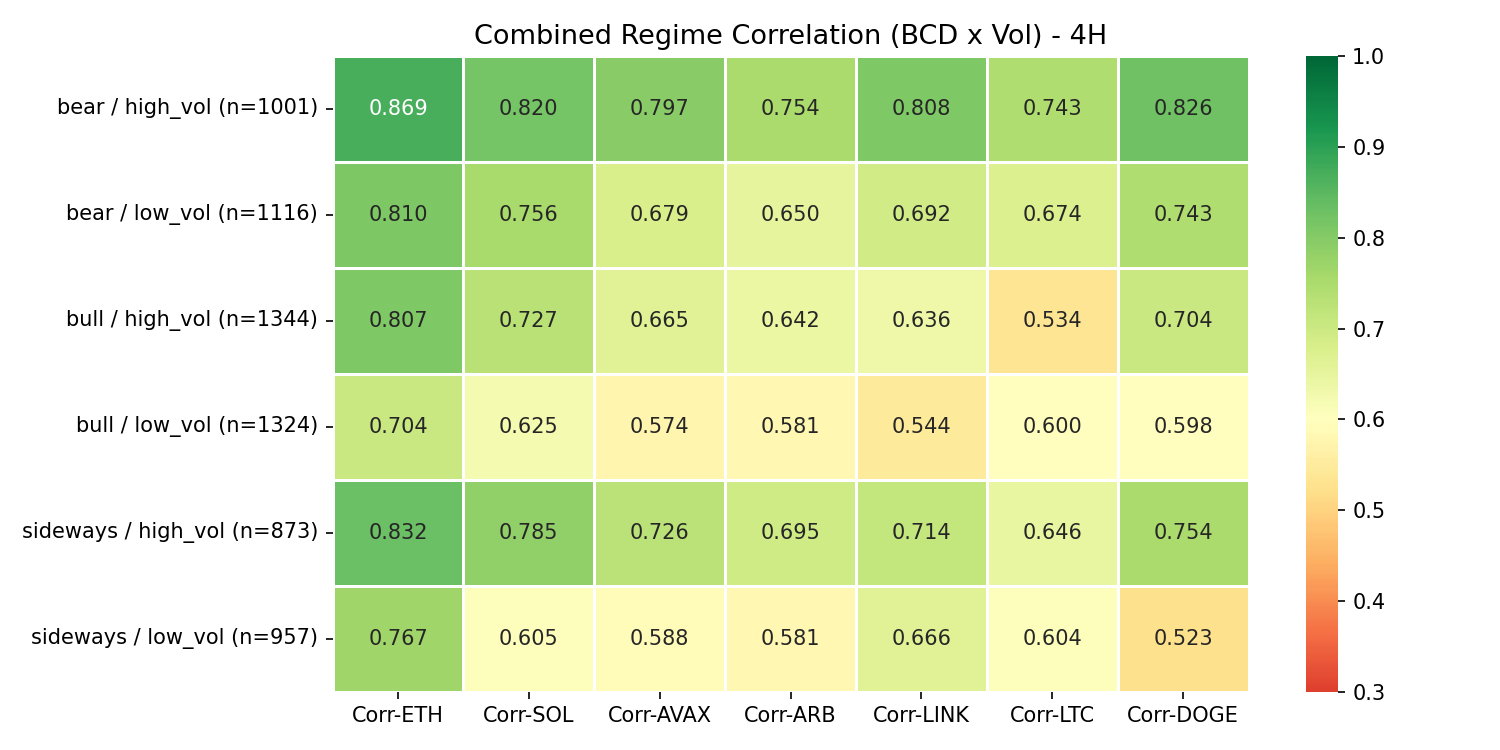
\includegraphics[width=0.85\linewidth,height=\textheight,keepaspectratio]{11_combined_regime_heatmap_4h.png}

}

\caption{\label{fig-combined-regime}Perbandingan korelasi (co-movement)
dan kemiringan regresi (Beta) untuk altcoin terpilih.}

\end{figure}%

\section{Analisis Lead/Lag}\label{analisis-leadlag}

Kami menyelidiki apakah ada altcoin yang bergerak lebih dulu sebagai
indikator awal BTC.

\begin{longtable}[]{@{}llll@{}}
\caption{Puncak lag CCF. Negatif artinya altcoin memimpin
BTC.}\label{tbl-ccf}\tabularnewline
\toprule\noalign{}
Pasangan & Puncak Lag (4H) & Puncak Lag (1D) & Temuan \\
\midrule\noalign{}
\endfirsthead
\toprule\noalign{}
Pasangan & Puncak Lag (4H) & Puncak Lag (1D) & Temuan \\
\midrule\noalign{}
\endhead
\bottomrule\noalign{}
\endlastfoot
ETH\(\to\)BTC & 0 & 0 & Simultann \\
ARB\(\to\)BTC & \(-7\) & \(-1\) & Noise Statistik \\
LTC\(\to\)BTC & \(-12\) & 0 & Noise Statistik \\
\end{longtable}

Meskipun ditemukan puncak lag negatif pada ARB dan LTC, uji
\textbf{Kausalitas Granger} mengonfirmasi bahwa pergerakan tersebut
tidak memiliki daya prediksi yang signifikan. Secara statistik, BTC
tetap merupakan pemimpin pasar (\emph{price leader}), sementara altcoin
seperti LTC (\(p = 0.004\)) dan DOGE (\(p = 0.033\)) secara signifikan
mengikuti pergerakan BTC.

\begin{figure}[htbp]

\centering{

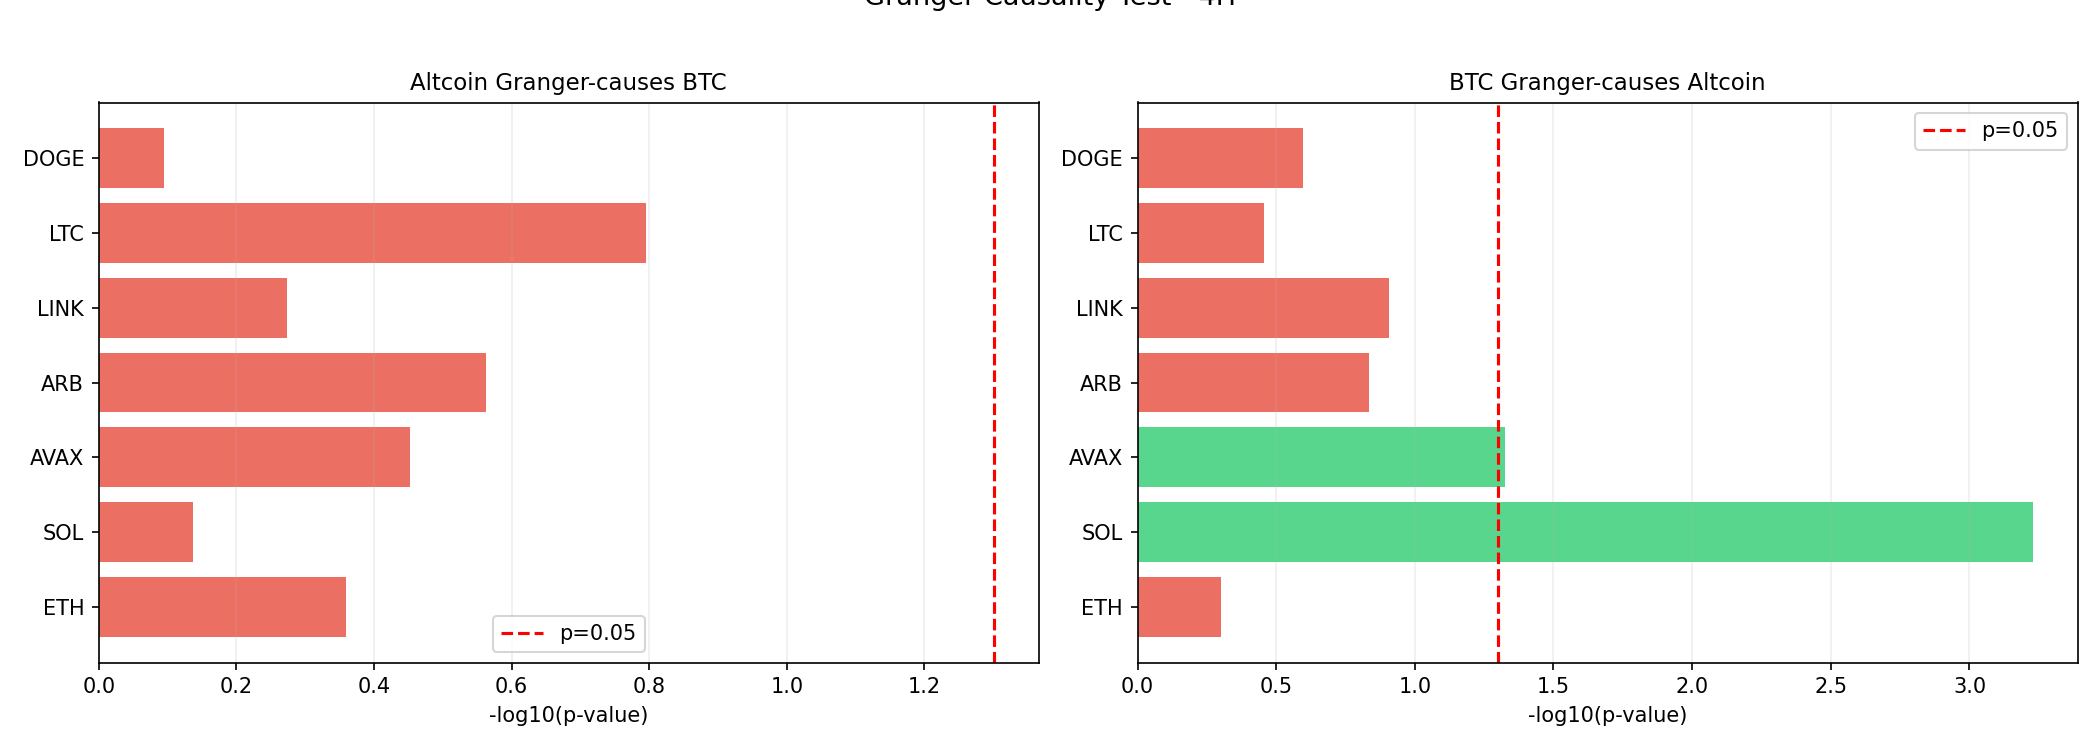
\includegraphics[width=0.85\linewidth,height=\textheight,keepaspectratio]{13_granger_4h.png}

}

\caption{\label{fig-granger}Hasil uji kausalitas Granger (4H).}

\end{figure}%

\section{Strategi Eksekusi Lintas Aset (Cross-Asset
Entry)}\label{strategi-eksekusi-lintas-aset-cross-asset-entry}

Berdasarkan temuan korelasi dan magnitudo (Beta), berikut adalah
strategi praktis untuk mengeksekusi altcoin menggunakan sinyal
BTC-QUANT:

\begin{enumerate}
\def\labelenumi{\arabic{enumi}.}
\tightlist
\item
  \textbf{Strategi Proksi Aman (Mirroring ETH):} Gunakan \textbf{ETH}
  sebagai aset utama untuk di-\emph{mirror} dari sinyal BTC. Dengan
  korelasi 0.82 dan Beta \textasciitilde1.1, ETH hampir selalu bergerak
  searah dengan BTC dengan risiko anomali yang sangat rendah.
\item
  \textbf{Strategi Amplifikasi Profit (High-Beta Entry):} Jika sinyal
  BTC-QUANT muncul pada \textbf{Rezim BCD Bear}, prioritaskan entri pada
  \textbf{ARB} atau \textbf{DOGE}. Karena Beta mencapai \textgreater{}
  1.5, keuntungan yang didapat bisa 50\% lebih besar dari pergerakan BTC
  dalam satu sinyal yang sama.
\item
  \textbf{Seleksi Aset Berbasis Rezim:} Jangan melakukan
  \emph{mirroring} ke altcoin (kecuali ETH) saat pasar berada di
  \textbf{Rezim Bull + Volatilitas Rendah}, karena korelasi turun
  drastis (\(r < 0.60\)). Pada kondisi ini, sinyal BTC seringkali gagal
  diikuti oleh altcoin.
\item
  \textbf{Validitas Pemicu (Trigger):} Karena uji \textbf{Kausalitas
  Granger} membuktikan BTC memimpin LTC dan DOGE, sinyal BTC adalah
  pemicu (\emph{trigger}) yang sah untuk melakukan entri tertunda pada
  altcoin tersebut.
\end{enumerate}

\section{Kesimpulan}\label{kesimpulan}

\begin{enumerate}
\def\labelenumi{\arabic{enumi}.}
\tightlist
\item
  \textbf{BTC adalah Trigger Universal} -- Riset membuktikan BTC adalah
  pemimpin harga (\emph{price leader}). Sinyal BTC-QUANT sangat valid
  untuk dijadikan pemicu entry di altcoin lain.
\item
  \textbf{ETH sebagai Bayangan BTC} -- Korelasi \(r=0.82\) menjadikan
  ETH aset termudah untuk di-\emph{mirror} dengan risiko ketidaksesuaian
  arah paling rendah.
\item
  \textbf{Pemanfaatan `Magnitudo' (Beta)} -- Untuk memaksimalkan profit
  dari satu sinyal BTC, \textbf{ARB, DOGE, dan AVAX} adalah pilihan
  utama karena sensitivitasnya yang tinggi (Beta \textgreater{} 1.4).
\item
  \textbf{Keunggulan Rezim Bear} -- Strategi \emph{cross-asset entry}
  paling efektif dilakukan saat pasar berada dalam \textbf{Rezim BCD
  Bear}, di mana seluruh ekosistem terkunci dalam korelasi yang sangat
  kuat (\(r \approx 0.90\)).
\end{enumerate}

Kesimpulan akhirnya: Sinyal BTC-QUANT dapat digunakan secara andal untuk
melakukan \emph{entry} pada altcoin guna mendapatkan keuntungan yang
lebih besar (melalui aset high-beta) atau melakukan diversifikasi proksi
yang lebih likuid.




\end{document}
